\documentclass[11pt, twoside, reqno]{book}
\usepackage{amssymb, amsthm, amsmath, amsfonts}
\usepackage[htt]{hyphenat}
\usepackage{graphicx}
\usepackage{color}
\usepackage{hyperref}
\usepackage{verbatim}
\usepackage{ wasysym }
\usepackage[toc,page]{appendix}
\appendixpageoff
\usepackage[leftmargin = 1in, rightmargin = 0in, vskip = 0in]{quoting}
\usepackage{microtype}
\usepackage{bardtex}
\biboption{amsrefs}
\styleoption{seniorproject}
\usepackage{listings}
\definecolor{codegreen}{rgb}{0,0.6,0}
\definecolor{codegray}{rgb}{0.5,0.5,0.5}
\definecolor{codepurple}{rgb}{0.58,0,0.82}
\definecolor{backcolour}{rgb}{0.95,0.95,0.98}
\lstdefinestyle{mystyle}{
    commentstyle=\color{codegreen},
    keywordstyle=\color{magenta},
    stringstyle=\color{codepurple},
    basicstyle=\ttfamily\footnotesize,
    backgroundcolor=\color{backcolour},
    frame=lrbt,
    breakatwhitespace=false,      
    framexleftmargin=8pt, 
    framexrightmargin=8pt,   
    framextopmargin=6pt,
    framexbottommargin=6pt,
    breaklines=true,                 
    keepspaces=false,                 
    numbersep=0pt,                  
    showspaces=false,                
    showstringspaces=false,
    showtabs=false,                  
    tabsize=1
}
\lstset{style=mystyle}
\newcommand{\blockquotespacing}{\blockspaced}
\newcommand{\prose}{.25in}
\newcommand{\poetry}{0in}
\newcommand{\singlespaced}{\setstretch{1}\vspace{\baselineskip}}
\newcommand{\blockspaced}{\setstretch{1.3}\vspace{\baselineskip}}
\newcommand{\doublespaced}{}
\newenvironment{blockquote}[1][\prose]{\setlength{\parindent}{#1}\begin{quoting}\blockquotespacing}{\end{quoting}}
\begin{document}
\startmain
\chapter{LDA Writeup}

Latent Dirichlet Allocation is a generative probabilistic unsupervised learning model popular in natural language processing (nlp). It is a generalization of ``probabilistic latent semantic analysis,'' and was created by David Blei, Andrew Ng, and Michael Jordon, and published as ``Latent Dirichlet Allocation'' in January 2003. As with some of their usage, we will be using this for text classification. In this sense, we can see the ideas behind LDA in its application to text classification with documents, topics, and words. A real document may discuss multiple topics, where related topics are likely to use similar words; this translates to the model where documents are assigned a topic mixture, where each topic is a distribution over the given corpus.

\subsection{Assumptions}

An LDA model naively assumes that documents are unordered lists (bags) of words, and that documents are unordered within a corpus, that is that word position nor document position affects output.

\subsection{Terminology}

We shall adopt the language of the original paper regarding the terms ``word,'' ``document,'' and ``corpus.'' A word is an item from a dictionary/vocabulary of words indexed by location; this allows for a word to be represented as a one-hot vector. For the dictionary $D = \left\{ \text{cat}, \text{dog}, \text{elephant} \right\}$, we would encode 'cat' as $\left[ 1, 0, 0 \right]$. A document is a sequence of words indexed by position, and a corpus is a bag of documents. As per LDA as a \textit{probabilistic model}, we view topics as hidden random variables. The following variables are relevant to LDA:

- $\alpha$: topic distribution by document, such that $\alpha_{ij}$ describes the probability of topic $j$ occurring within document $i$. A higher $\alpha$ corresponds to documents being comprised of more topics, as alpha approaches 0, we see this mixed membership model (document belongs to many topics) approach a mixture model (document belongs to one topic)

- $\beta$: word distribution by topic, such that $\beta_{ij}$ describes the probability of word $j$ belonging to topic $i$. A higher $\beta$ corresponds to topics being comprised of more words

- $\theta$: topic distribution for a given document, such that each $\theta_i > 0$  and $\sum_{i=0}^{k} \theta_i=1$

- $z$: topic for a given word within a given document

- $w$: word within a given document

\subsection{A Graphical Representation}

\begin{figure}[h!]
    \centering
    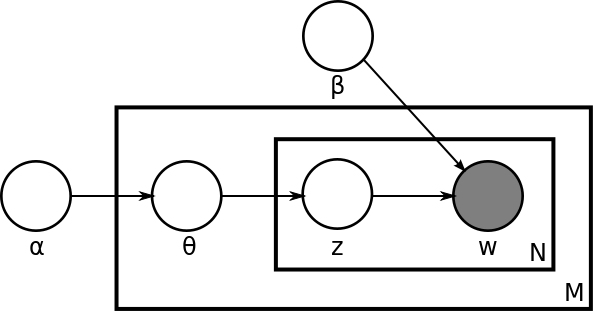
\includegraphics[width=15cm, height=6cm, keepaspectratio]{/Users/colehollant/Projects/sproj/resources/lda-not-verbose.png}
    
    \href{https://upload.wikimedia.org/wikipedia/commons/thumb/d/d3/Latent_Dirichlet_allocation.svg/593px-Latent_Dirichlet_allocation.svg.png}{Plate diagram for LDA}
\end{figure}


Within the classic plate diagram for LDA, we have $M$ documents, $N$ topics, and an unlabelled vocabulary $V$. We take the topic distribution $\theta$, a $K$-dimensional random variable, as drawn from a Dirichlet distribution, $\alpha$. On the other end, $\beta$ is a $K \times V$ matrix for a vocabulary of size $V$ that defines the word-topic probabilities. Arrows between nodes represent dependency, and $w$ is the sole darkened node as it is the only observed variable, all others are latent.

\subsection{LDA Overview}

With probabalistic latent semantic indexing, an occurence of a word is modeled as a sample from a topic mixture, leading to a probability distribution on a set of topics. Ng, Blei, and Jordan sought to extend this to account for document-level probabilities. Documents are mixtures with latent topics that are defined by a distribution of words.

With LDA, we are able to fix some number of topics, $K$, of which to determine; we can do this via collapsed Gibbs sampling. We begin with a random assignment of words in each document to topics $Z_{0\dots K}$ from a Dirichlet distribution as some initial document-topic representation and as some defined word-distribution for each topic.

From here, we fall into a training loop. We consider each document $d$, and each word $w$ within each document, we must compute $p(t | d)$ as well as $p(w | t)$ for each topic $t$. Then we will reassign $w$ to a topic, $t$, with probability $p(t | d) \cdot p(w | t)$, or the probability that $t$ has generated $w$. Note that the reassignment step assumes all word-topic distributions to be correct except for that of $w$. Once we reach convergence, or exhaust a defined number of epochs, we hope to see reasonable word-topic and document-topic distributions, which we can use to infer topic mixtures of documents.

Determining the probability of a topic given a word is an application of Bayes theorem:

$$p(t | w) = \frac{p(w | t)\cdot p(t)}{p(w)}$$

where we know the probability of a word (as informed by our corpus), the probability of a topic being chosen, and the probability of a word given a topic (as informed by the model state). Bear in mind, this has been glossed over as we did not focus on the implementation, for further reading, one should read \href{http://www.ccs.neu.edu/home/vip/teach/DMcourse/5_topicmodel_summ/notes_slides/sampling/darling-lda.pdf}{Darling}, or \href{http://jmlr.csail.mit.edu/papers/v3/blei03a.html}{Blei et al.}.
\end{document}